\chapter{Graphs}
\label{chp:graphs}
In this chapter are introduced the fundamentals concepts of \textbf{graphs} as mathematical objects, and as an abstract data type, its applications in computer science, and the most important and notable algorithms with their implementation. 
 
\section{General Definitions}
A graph is a discrete mathematical structure in which the connections between its elements, and their relationship are highlighted. A graph is made up by two different elements: \textbf{nodes} or \textbf{vertices}, and \textbf{links} or \textbf{edges}. In case the links do not have any direction the graph is called \textbf{undirected graph} (Figure), in case instead the links have a direction the graph is called \textbf{directed graph}.

\begin{figure}[H]
	\begin{center}
		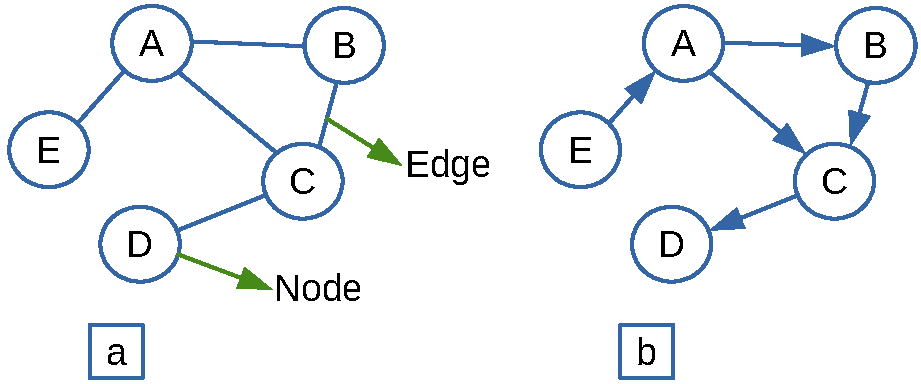
\includegraphics[scale=.6]{chapters/graphs/images/graphs_1.pdf}
		\caption[Undirected (a) and directed (b) graphs and its elements.]{Undirected (a) and directed (b) graphs and its elements.}
		\label{graphs_1}
	\end{center}
\end{figure}

Formally a graph is the pair \(G=(V, E)\), where \(V\) is the set of all vertices, and \(E\) is the set of paired vertices, whose elements are called edges \cite{wikigraphmath} (\href{https://en.wikipedia.org/wiki/Graph_(discrete_mathematics)}{Graph, Wikipedia}).

A \textbf{tree} (Chapter \ref{chp:trees}) is a special kind of graph.

Graphs are very useful to describe a lot of real situations like: connections between people, computers (internet), web pages (world wide web), airports, cities, and gene inside the DNA.

In graphs, differently to trees, closed loops can exist. These kind of closed loops can be dangerous for the algorithms because they could lead to infinite executions.

\subsection{Connectivity}
\textbf{Connectivity} is a measure that describe how much the nodes of a graph are connected. It is defined as the minimum number of elements (nodes or edges) that need to be removed to separate the remaining nodes into isolated subgraphs \cite{wikiconnectivity} (\href{https://en.wikipedia.org/wiki/Connectivity_(graph_theory)}{Connectivity, Wikipedia}).

A graph is said to be \textbf{connected} if every pairs of nodes are connected. Thus it always exists at least one path that connects every pairs of nodes. If an undirected graphs is not connected then it is \textbf{disconnected}: in this case there is one or more nodes that can not be reached by any paths.

\paragraph{Strongly Connected}
A directed graph is said to be \textbf{strongly connected} if every pairs of nodes can be reached by one or more path.

\paragraph{Weakly Connected}
A directed graph is said to be \textbf{weakly connected} if by replacing all the direct edges with undirectd ones, the new graph is connected. in a directed graph some nodes can not be reached if all the edges exit or enter from them. The graph in Figure \ref{graphs_2} is weakly connected because the node \(U\) has only entering edges.

\begin{figure}[H]
	\begin{center}
		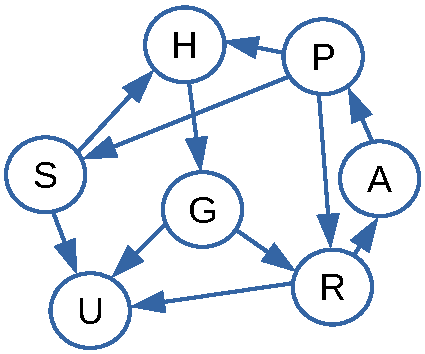
\includegraphics[scale=.6]{chapters/graphs/images/graphs_2.pdf}
		\caption[A weakly connected graph.]{A weakly connected graph.}
		\label{graphs_2}
	\end{center}
\end{figure}

\section{Graph Representations}
There are several ways to represent graphs using data structures. For example in an object oriented programming language a way could be to define a type for the vertex, and a type for the edges.

The most common data structures used for representing a graph are: \textbf{edge list}, \textbf{adjacency list}, and \textbf{adjacency matrix} \cite{goodrich2013data}. 

In appendix \ref{graphsappendix} there is a summary of the complexities for the most common operations performed on graphs for the different data structures.

\subsection{Edge List}
The \textbf{edge list} is an unordered list of all pairs of nodes that form an edge. This representation is minimal but it does not allow to locate a specific edge, or the set of edges incident to a particular node \cite{goodrich2013data}.

\begin{figure}[H]
	\begin{center}
		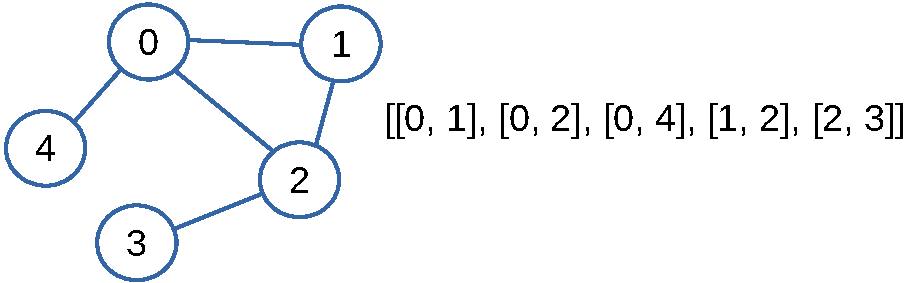
\includegraphics[scale=.6]{chapters/graphs/images/graphs_3.pdf}
		\caption[Edge list.]{Edge list.}
		\label{graphs_3}
	\end{center}
\end{figure}

\subsection{Adjacency List}
The \textbf{adjacency list} is a list containing a separate list for each node containing all the incident edges of that node. In this representation identify all the edges incident to a node is easy \cite{goodrich2013data}. In case of directed graphs for each node there are two different lists: one for entering edges, and another one for the edges that go out.

\begin{figure}[H]
	\begin{center}
		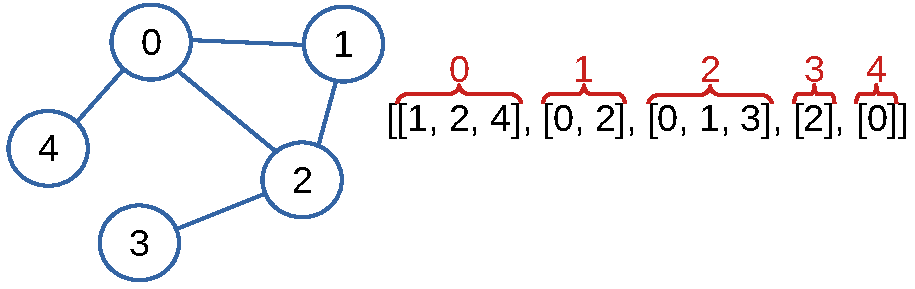
\includegraphics[scale=.6]{chapters/graphs/images/graphs_4.pdf}
		\caption[Adjacency list.]{Adjacency list.}
		\label{graphs_4}
	\end{center}
\end{figure}

\subsection{Adjacency Matrix}
The \textbf{adjacency matrix} is a matrix \(A\) in which each element \(A[i, j]\) represent the relationship between the edge \(i\) with the edge \(j\). If between \(i\) and \(j\) there is an edge \(A[i, j] = 1\), otherwise \(0\). In case the an ed go out and enter in the same edge \(A[i, i] = 1\). For undirected graphs this matrix is symmetric, and in case there are not edges going in and out the same node the principal diagonal is all of \(0\).

\begin{figure}[H]
	\begin{center}
		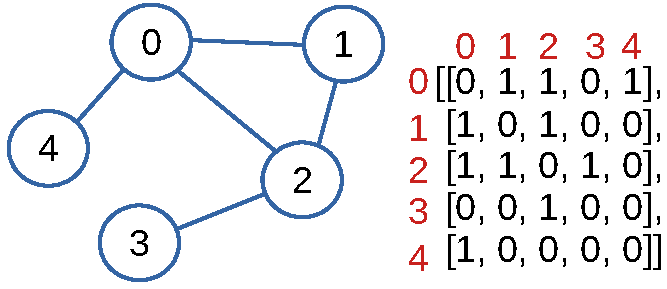
\includegraphics[scale=.6]{chapters/graphs/images/graphs_5.pdf}
		\caption[Adjacency matrix.]{Adjacency matrix.}
		\label{graphs_5}
	\end{center}
\end{figure}

In the appendix \ref{graphimplementationappendix} there is the full python implementation of the graph representation. There are defined the classes for nodes, edges, and graphs objects. Moreover, all the main operations on graphs like: insert a new node, a new edge, get the edge list, the adjacency list, the adjacency matrix, and find the max index are also implemented.

\section{Graph Traversal}
Like in the case of trees (Chapter \ref{chp:trees}), also for graphs there are two different way to traverse the structure: \textbf{depth-first search}, and \textbf{breadth-first search}. But for graphs, differently from trees, there is not a privileged way to traverse the structure. Then it is arbitrarily choose a node where to start the search.

\subsection{Depth-first Search (DFS)}

\subsection{Breadth-first Search (BFS)}